\documentclass[main.tex]{subfiles}
\begin{document}

\section{Astronomical measurements through the ages}

Astronomy has historically been among the first of the \emph{exact sciences}, 

\subsection{Pre-magnification angle measurement}

\subsection{Modern era improvements}

The accuracy of angular measurements skyrocketed in the modern era: between the 1500s and the 1800s there was roughly an order of magnitude improvement in accuracy per century \cite[]{chapmanAccuracyAngularMeasuring1983}.


\subsection{Current state of the art}

The limit nowadays, for space-based instruments like the Hubble Space Telescope which are not affected by the atmosphere, is the intrinsic wavelike nature of light: the equation for the \emph{diffraction limit} is 
%
\begin{align}
\theta \approx \num{1.22} \frac{\lambda }{D}
\,,
\end{align}
%
where \(\theta \) is the minimum angular distance of two points we can distinguish,\footnote{This is to be interpreted in the precise sense that two points are \emph{distinguished} if the first diffraction minimum of one coincides with the peak of the diffraction pattern of the other.} \(D\) is the diameter of our telescope, while \(\lambda \) is the wavelength of the light we are considering.
For example, the HST has a diameter of \SI{4.2}{m}, so for visible green light at \SI{500}{nm} its diffraction limit is of around \SI{30}{mas} (milli-arcseconds).
Beyond this limit objects cannot be resolved. 

\section{Equinox precession as a dating tool}

The Earth's axis of rotation is tilted by an angle of around \SI{24}{\degree} with respect to the \emph{ecliptic}, which is the plane in which the Earth's orbit around the Sun lies. 

In the time it takes for the Earth to complete a revolution around the Sun the orientation of this axis with respect to the distant stars is roughly constant --- this can be seen easily in the night sky from the fact that the sky appears to revolve around a fixed axis, which in the Northern Hemisphere is close to the star Polaris.\footnote{Currently the separation of the star from the northern celestial pole --- which corresponds to \(\SI{90}{\degree} - \delta \), where \(\delta \) is the declination of Polaris in an equatorial coordinate system at a chosen equinox --- is around \SI{39}{^\prime}, and it is decreasing, it will reach a minimum of \SI{27}{^\prime} in the year 2102DC \cite[pag.\ 58]{barbieriLezioniDiAstronomia2003}.}

However, it was noticed as early as 129BC by Hypparcos that the axis of rotation does not remain stationary over the years. 

In an ecliptic coordinate system we find that the ecliptic latitude of stars stays constant, while their ecliptic longitude increases by around \SI{50.3}{\arcsec} per year, which corresponds to a full revolution every \SI{25772}{yr}.
This motion is called the \emph{precession of the equinoxes}
\cite[]{barbieriLezioniDiAstronomia2003}. 

Because of it, the Celestial North Pole appears to rotate clockwise around the Ecliptic North Pole. The appearance of the ecliptic grid in the modern night sky is shown in figure \ref{fig:ecliptic-grid}. 

\begin{figure}[ht]
\centering
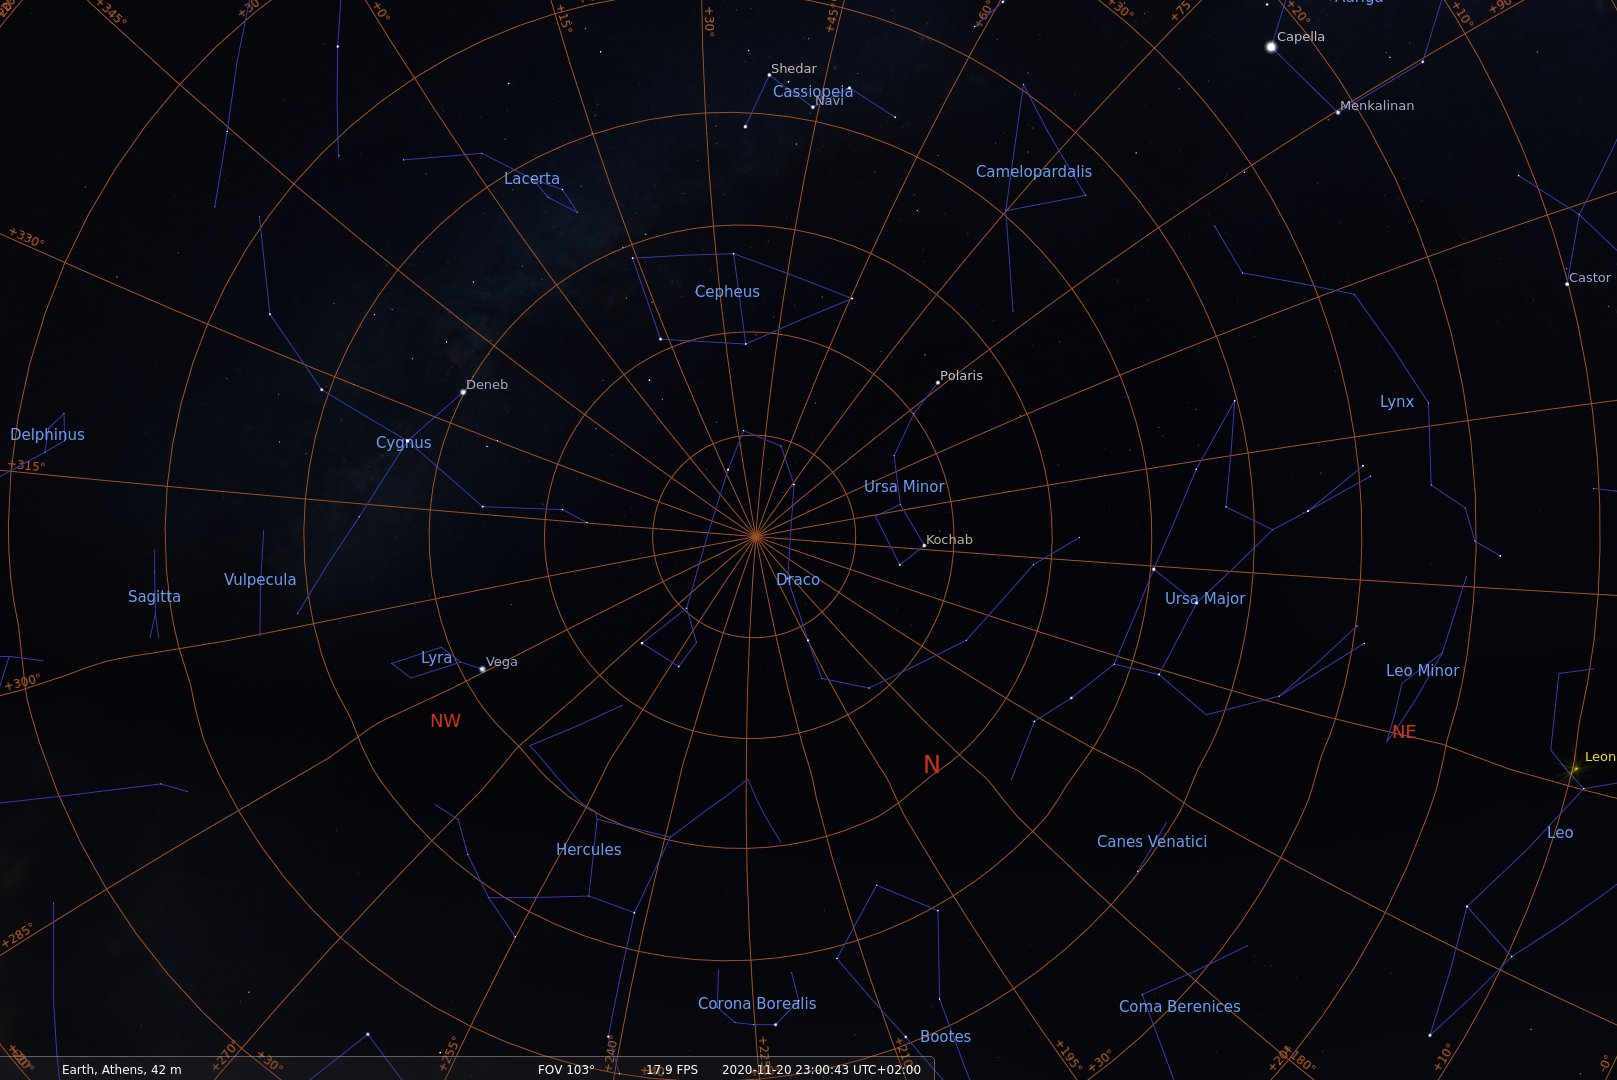
\includegraphics[width=\textwidth]{figures/ecliptic_grid_athens_now.png}
\caption{Ecliptic grid on the night sky in 2020. One can see that the Ecliptic North Pole is situated in the constellation of Draco, around \SI{24}{\degree} away from the Celestial North Pole. Image created in Stellarium \cite[]{stellariumcontributorsStellariumAstronomySoftware2020}.}
\label{fig:ecliptic-grid}
\end{figure}

This means that the appearance of the night sky changes over the centuries in a way that is detectable even without high angular precision measurements. 

\subsection{Dating the Farnese Atlas}

The Farnese Atlas is a Roman statue from the second century AD, depicting the Titan Atlas who, after the Titanomachy (the war of the Titans against the Olympians) was punished by Zeus with the task of holding up the sky.

He is depicted as a hunched, muscular man holding up the celestial sphere. On the sphere is a map of constellations, as well as several important circles: the celestial equator, the Tropics of Cancer and Capricorn, the Artic and Antarctic Circles; the equinoctial and solstitial colures \cite[table 4]{schaeferEpochConstellationsFarnese2005}. 

Art historians had long debated the source of the positions of the sculpted constellations, with potential references dating from 1150BC to 150AD; a 2005 study by \textcite[]{schaeferEpochConstellationsFarnese2005} allowed for the matter to be settled: the positions of the stars refer to the year 125BC, \(\pm \SI{55}{yr}\) (at \SI{68}{\percent} C.\ L.).

This matches very well with the stars' positions being taken from the catalog by Hipparchus, who indeed lived in the second century BC. 
The finding is further corroborated by several details about the constellation being only consistent with Hipparchus' work \cite[sec.\ 2]{schaeferEpochConstellationsFarnese2005}.

How was the confidence interval calculated? First, Schaefer accurately measured the position of the recognizable points in the constellations from photographs of the Atlas taken at a known distance.
From these positions we can determine the epoch of the atlas: if the incisions were precisely accurate, we could only look at the position of the vernal equinox (whose right ascension is clearly marked by the presence of the colure on the atlas).

On the Atlas, the constellation of Aries (the Ram) ends precisely on the colure, so we can tell that the sky would have looked roughly as in figure \ref{fig:aries}, which refers to the year 184BC. 

% This allows us to make a first order-of-magnitude estimate. The position of the equinox compared to the 

\begin{figure}[ht]
\centering
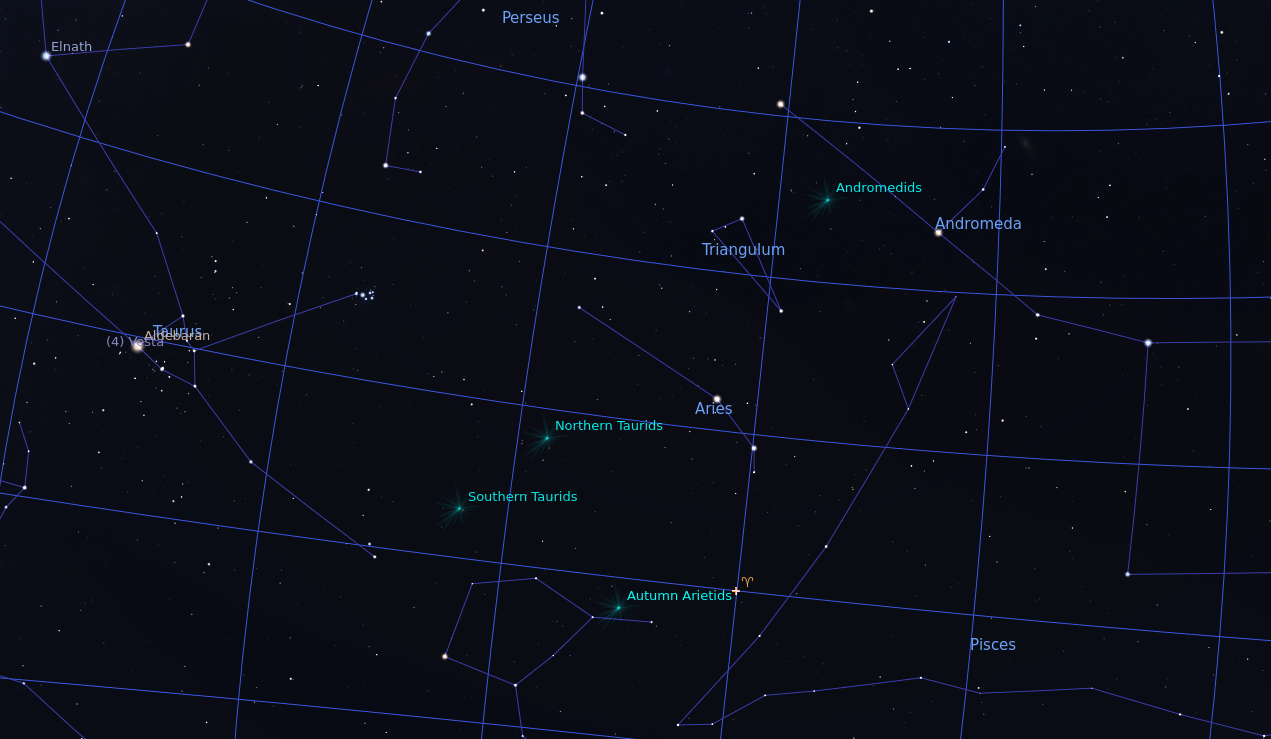
\includegraphics[width=\textwidth]{figures/aries_on_colure_184_BC.png}
\caption{The constellation of Aries is shown, as well as the vernal equinox, on an equatorial grid; this is how the sky would have looked in 184BC. The colure is the vertical line passing by the equinox (marked as \(\aries\)), and one can see that it passes by the right side of Aries; this is what appears in the Farnese Atlas.}
\label{fig:aries}
\end{figure}

This, however, is too imprecise. A detailed analysis of the positions of all the stars shows that they are incompatible among themselves, in a way which is compatible with a Gaussian random error on the position of each point. The standard deviation of this Gaussian is roughly \SI{3.5}{\degree} for the points which lie on the aforementioned celestial circles, and \SI{5}{\degree} for ones which do not. 
% These positions are compared among themselves 

This might seem like a rather large error to be able to draw any kind of conclusion.
Indeed, we can directly relate this accuracy to an uncertainty in years using the rate of precession of the equinoxes, \SI{50.3}{\arcsec / yr}: a \SI{3.5}{\degree} uncertainty on the position of a star corresponds to a \SI{250}{yr} uncertainty in the epoch. 
Fortunately, we can measure the position of more than one star, and roughly speaking measuring \(N\) of them reduces the error by a factor \(\sqrt{N}\). 

Schaefer measured \(N = 70\) different points, and employed a \(\chi^2\) minimization procedure in order to find which year corresponded to the least global error in positioning of the constellations, which yielded the final estimate for the epoch of the catalog from which the constellations were drawn. 

The uncertainty of the positions must have been due to both intrinsic errors in the original catalog, and mistakes or imprecision by the sculptor.
Because of this, Schaefer estimates the precision of Hipparchus' atlas to have been \(\lesssim \SI{2}{\degree}\).

\subsection{Ursa Maior in the Iliad}

The following passage of the Iliad appears in the description of the magnificent shield wrought by Hephaestus for Achilles in order for him to go avenge Patroclus, who was slain by Hector.
On the shield, among other things, are depicted the constellations \cite[XVIII, 483--490]{murrayIliad1924}: 
%
\begin{quotation}
``Therein he wrought the earth, therein the heavens therein the sea, and the unwearied sun, and the moon at the full, and therein all the constellations wherewith heaven is crowned—the Pleiades, and the Hyades and the mighty Orion, and the Bear, that men call also the Wain, that circleth ever in her place, and watcheth Orion, and alone hath no part in the baths of Ocean.''
\end{quotation}

\begin{figure}[ht]
\centering
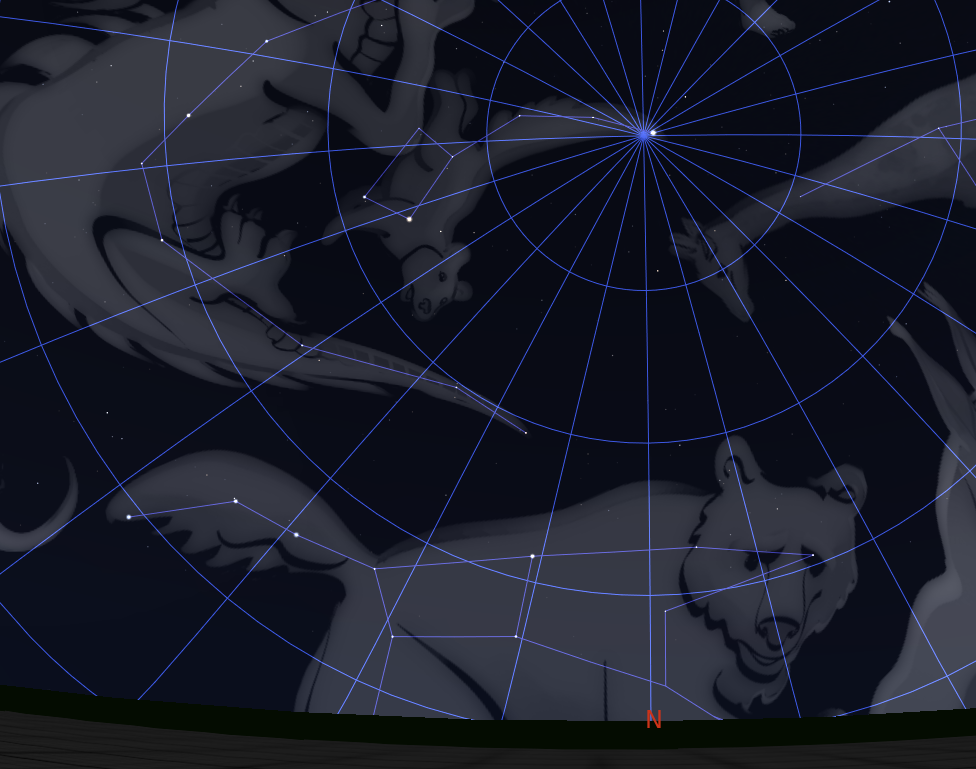
\includegraphics[width=\textwidth]{figures/ursa_maior_today.png}
\caption{The constellation of Ursa Major as seen in 2020 from Athens, Greece \cite[]{stellariumcontributorsStellariumAstronomySoftware2020}.}
\label{fig:ursa-now}
\end{figure}

Homer (or whoever wrote the Iliad) is stating that the Bear --- Ursa Maior, also known as the Wain (which means ``Cart'') --- alone never ``bathes in the Ocean'', meaning that it never goes below the horizon. 

This statement has a close connection to the latitude and epoch at which the observations leading to the passage were made. 
If one is at a latitude \(\varphi \) in the Northern Hemisphere, then they will see the North Celestial Pole at an altitude of \(\varphi \) above the horizon. In the night the sky will appear to rotate around the NCP, and stars whose declination is \(\delta \geq \SI{90}{\degree} - \varphi \) will appear never to set below the horizon. 

In figure \ref{fig:ursa-now} one can see how the Great Bear will appear in the night sky of 2020 from Athens: the ``Big Dipper'' asterism hardly sets, but it only represents the body of the bear, whose legs definitely go below the horizon. 

\begin{figure}[ht]
\centering
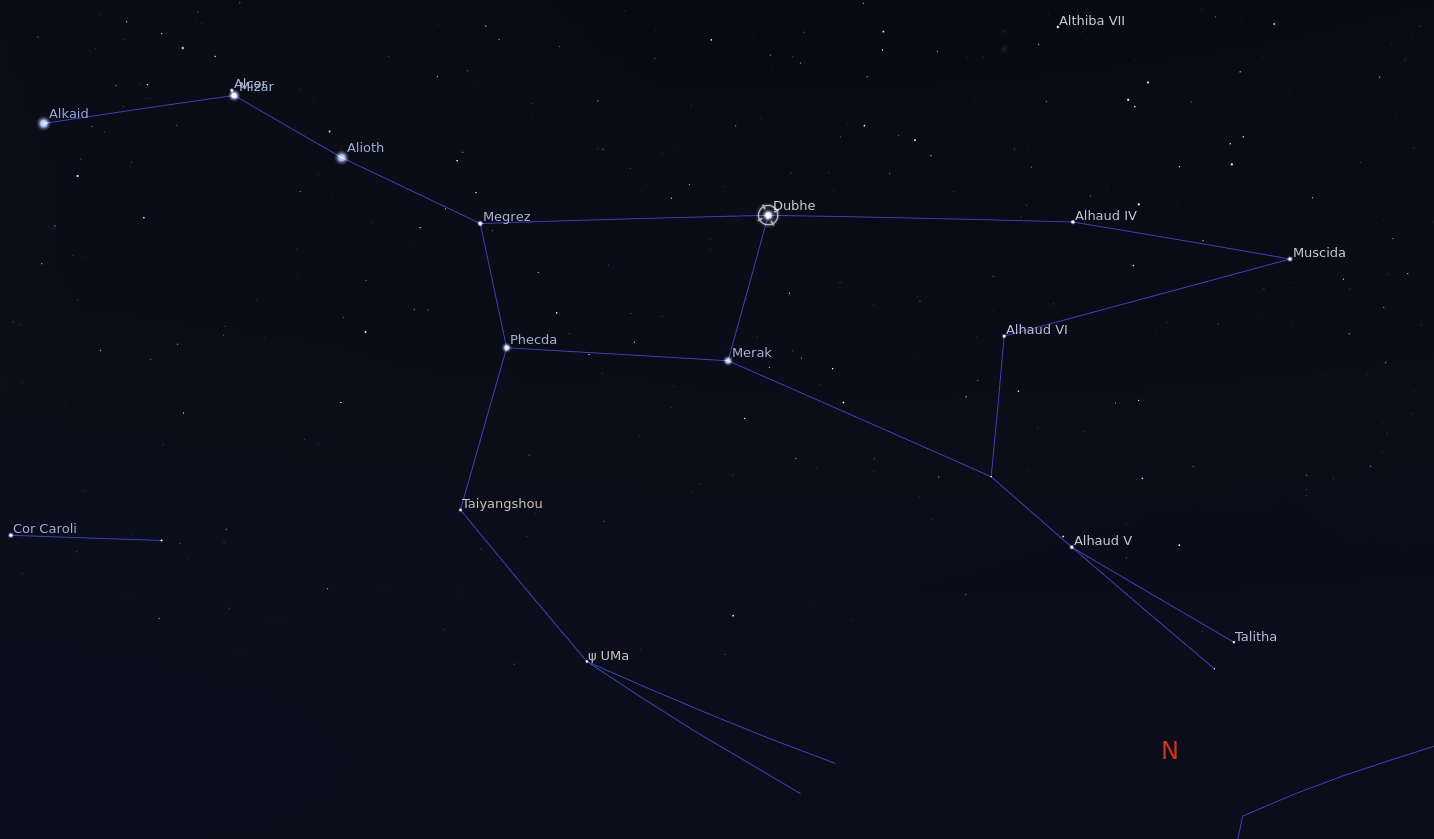
\includegraphics[width=\textwidth]{figures/ursa_names.png}
\caption{Ursa Major: names of all the main stars in the constellation \cite[]{stellariumcontributorsStellariumAstronomySoftware2020}.}
\label{fig:ursa-names}
\end{figure}


\begin{figure}[ht]
\centering
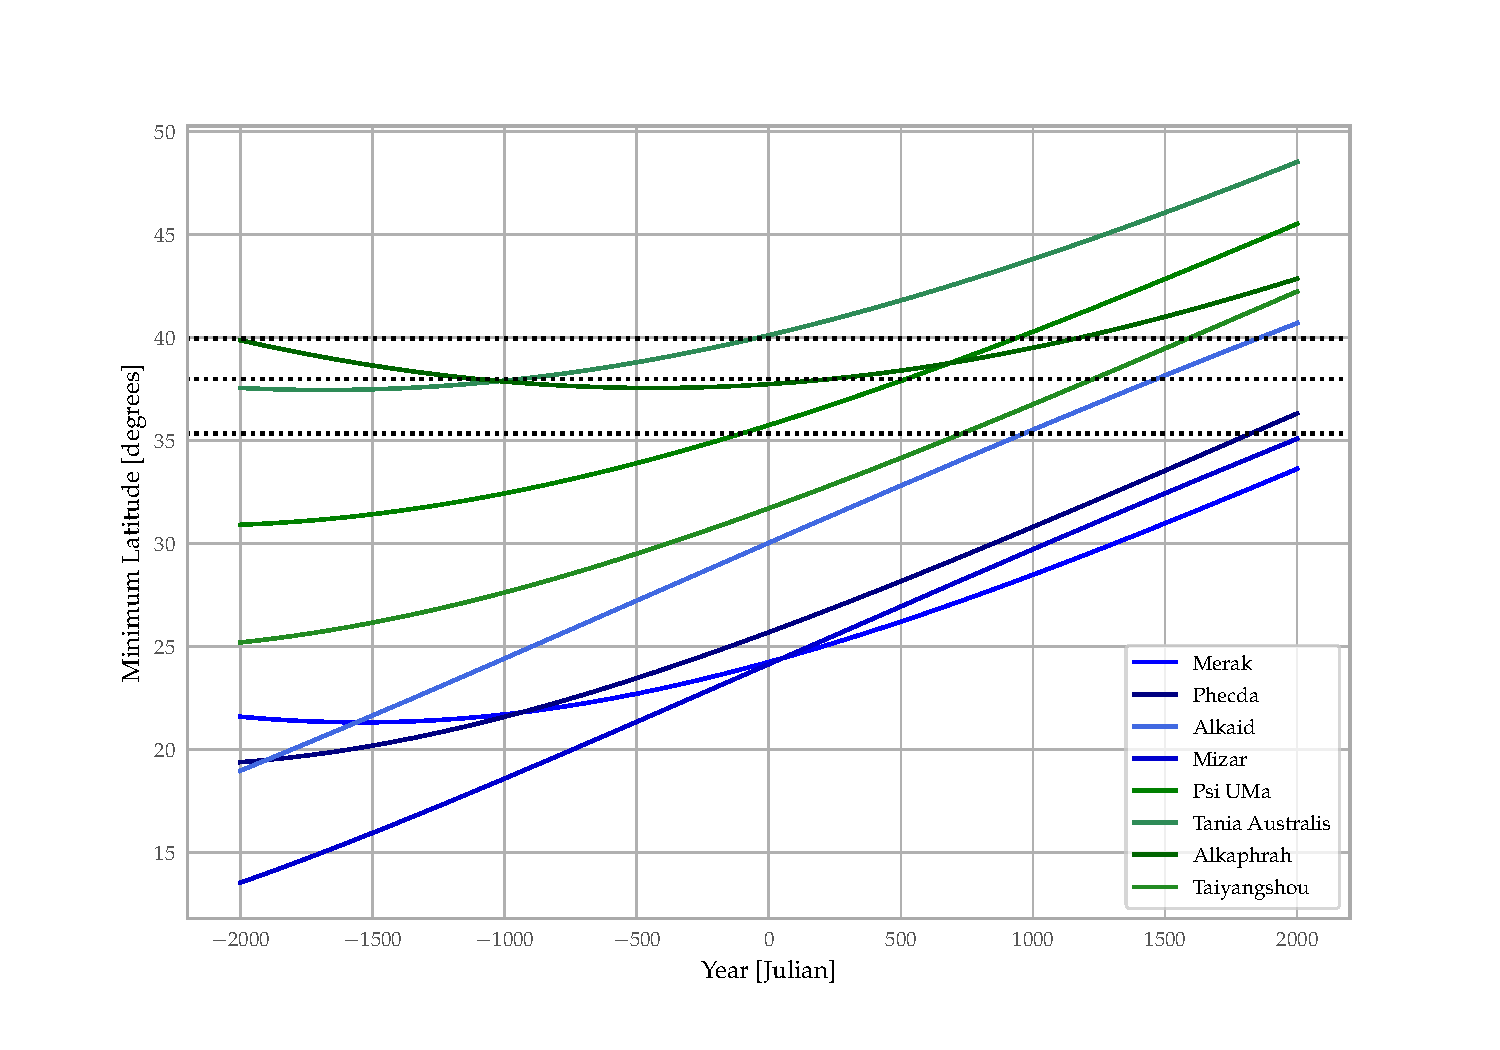
\includegraphics[width=\textwidth]{figures/Ursa.pdf}
\caption{The minimum latitude at which certain selected stars from the constellation of Ursa Maior would have appeared not to touch the horizon at varying times, from 2000BC to 2000AD. Stars from the Wain are shown in blue, stars from the ``legs'' of the bear are shown in green. Shown as dotted black lines are the latitudes of Troy, Athens and Crete (in order, from top to bottom).}
\label{fig:ursa}
\end{figure}

\end{document}
